%% Exemplo de como usar a classe ppgccufscar.
%% O template da monografia (quali, dissertacao ou tese)
%% foi feito pela Profa. Sandra Fabbri.
%% A classe ppgccufscar foi feita por Daniel Beck,
%% Daniel Bruno e Prof. Marcio


%%
%% Opcoes que podem ser passadas 'a classe
%%
%% Todas as opcoes da classe abnt (AbnTeX) sao validas.
%% Outras opcoes sao: quali e tese (dissertacao e' padrao)
%%

\documentclass[qualidoc]{ppgccufscar}

%% pacotes que deseja usar
%% pacotes incompativeis sao:
%%   qualquer pacote de citacoes, como natbib, apalike, cite, etc.
%% o pacote babel ja vem carregado com ingles e portugues
\usepackage[latin1]{inputenc}
\usepackage{enumerate}
\usepackage{graphicx}
\usepackage{multirow}
% \usepackage[T1]{fontenc}

\usepackage{url}
% \usepackage[a4paper,landscape]{geometry}
\usepackage{lscape}

% \usepackage{hyperref} 
% \hypersetup{colorlinks=false}

\usepackage[table]{xcolor}
\usepackage{colortbl}
%colorir linhas da tabela

\newcommand{\profileSpec}{\textit{Perfil-Especialista}}
\newcommand{\profileMPS}{\textit{Perfil-MPS.Br}}
\newcommand{\profileTMMi}{\textit{Perfil-TMMi}}

\usepackage{color}
\newcommand{\fabiano}[1]{{\color{blue} #1}}
\newcommand{\kamilla}[1]{{\color{black} #1}}
\newcommand{\sandra}[1]{{\color{red} #1}}


\titulo{T�tulo}
\autor{Priscilla de Abreu Lopes}
\orientador[Orientadora]{Profa. Dra. Heloisa de Arruda Camargo}
% \co-orientador{Prof. Dr. Fabiano Ferrari}
\areaconcentracao{Intelig�ncia Artificial}
\data{Mar�o/2014}

% epigrafre, agradecimentos sao feitos 'na mao'.
% um dia eu faco alguns comandos para eles ;)

\begin{document} 


\capa
\folhaderosto

%\dedicatoria{.........}

%\begin{agradecimentos}
%Agrade�o ao \LaTeX por n�o ter v�rus de macro.
%Agrade�o ao Linus Torvalds por ter feito o Linux.
%Agrade�o ao Bill Gates por deixar-nos piratear seus softwares.
%\end{agradecimentos}

%\epigrafe{texto}{autor}

\begin{resumo}


\textbf{Contexto:} ...
\textbf{Objetivo:} ... 
\textbf{Metodologia:} ...
\textbf{Resultados:} ...
\textbf{Conclus�es:} ...


\palavraschave{teste de software, melhoria de processo, TMMi, defini��o de processo, empresas de pequeno porte}

\end{resumo}



\begin{abstract}

....

\keywords{...}

\end{abstract}

\listoffigures
\listoftables

%% sumario
\tableofcontents

%% aqui comeca o texto da monografia
%% voce pode dividir o conteudo em varios arquivos.
%% por exemplo, intro.tex, fundamentacao.tex, desenvolvimento.tex, conclusao.tex.
%% dai, vc inclui aqui assim: As técnicas clássicas de AM consideram particularidades para os dados disponíveis: assume-se que o conjunto de exemplos é finito e que os exemplos seguem uma distribuição estática e estão disponíveis para acesso sempre que necessário durante o processo de aprendizagem. 

A evolução e ampliação do acesso a novas tecnologias e a internet tornaram propício o surgimento e desenvolvimento de diferentes e novos domínios para os quais as características assumidas pelas abordagens clássicas de AM não são verdadeiras.

Existe hoje uma variedade de sistemas que produzem grande quantidade de dados em curto espaço de tempo, como monitoração de tráfego de rede \cite{Aggarwal2008,Yu2009,Zhang2012,Breve2013}, redes de sensores \cite{gama2007,Pan2007,Zhang2012,Bouchachia2014}, mineração de \emph{clicks} na \emph{web} \cite{Marin2013}, medida de consumo de energia \cite{DeSilva2011,Zhang2012}, fraude de cartão de crédito \cite{wu2012}, mineração de textos da \emph{web} \cite{FdezRiverola2007,Cheng2011,Kmieciak2011,Nahar2014}, rastreamento visual \cite{Liu2014}, olfação artificial \cite{DeVito2012}, pesquisa meteorológica, mercado de ações e registros de supermercados \cite{Yogita2013}.

Sistemas como os citados impulsionaram a pesquisa por técnicas de aprendizado capazes de lidar com as peculiaridades desses novos domínios: tamanho indefinido, potencialmente infinito, e podem gerar exemplos com distribuição estatística mutável de acordo com o tempo \cite{Gama2010}. Nesse contexto teve origem uma nova abordagem denominada Aprendizado em Fluxo de Dados (AFD).

No modelo de Fluxo de Dados (FD) alguns ou todos os exemplos de entrada que serão utilizados não estão disponíveis em disco ou memória para acesso a qualquer momento, mas surgem de maneira contínua, em um ou mais fluxos. FDs diferem de conjuntos de exemplos ditos convencionais em diversos aspectos \cite{Babcock2002}:

\begin{itemize}
\item Os exemplos no fluxo chegam de maneira contínua e constante;
\item O sistema não possui controle sobre a ordem na qual os exemplos chegam para serem processados;
\item Os fluxos têm tamanho potencialmente infinito;
\item Uma vez que um exemplo do FD foi processado, ele é descartado ou arquivado. Estes exemplos não podem ser recuperados de forma simples, pois guardá-los em memória ou disco seria inviável.
\end{itemize}

Devido às limitações de tempo e espaço que ocorrem por causa das peculiaridades de FDs, as técnicas de AFD devem considerar que encontrar conhecimento válido de maneira rápida é uma prioridade para esses domínios, mesmo que o encontrado seja uma aproximação do obtido caso fosse possível ter o conjunto de exemplos completo para a aplicação de AM clássico. e assim por diante.

% \chapter{Introdu��o}

Este cap�tulo introduz o contexto e a motiva��o que levaram � elabora��o de uma proposta ...

Teste de Acr�nimo (TdA)\acronym{TdA}{Teste de Acr�nimo}

\section{Contexto e Motiva��o}

Exemplos de cita��o:

\begin{itemize}
  \item Normal: \cite{Rodrigues2010}
  \item Autores fora dos par�nteses: \citeonline{Rodrigues2010}
\end{itemize}






% \chapter{Outro Cap�tulo}


Este cap�tulo...



\section{Exemplo de Se��o}

Exemplo de figura: Na Figura~\ref{fig:chartsProfiles} ilustra-se ...


\begin{figure}[!ht]
%\begin{figure}[t]
  \centering
  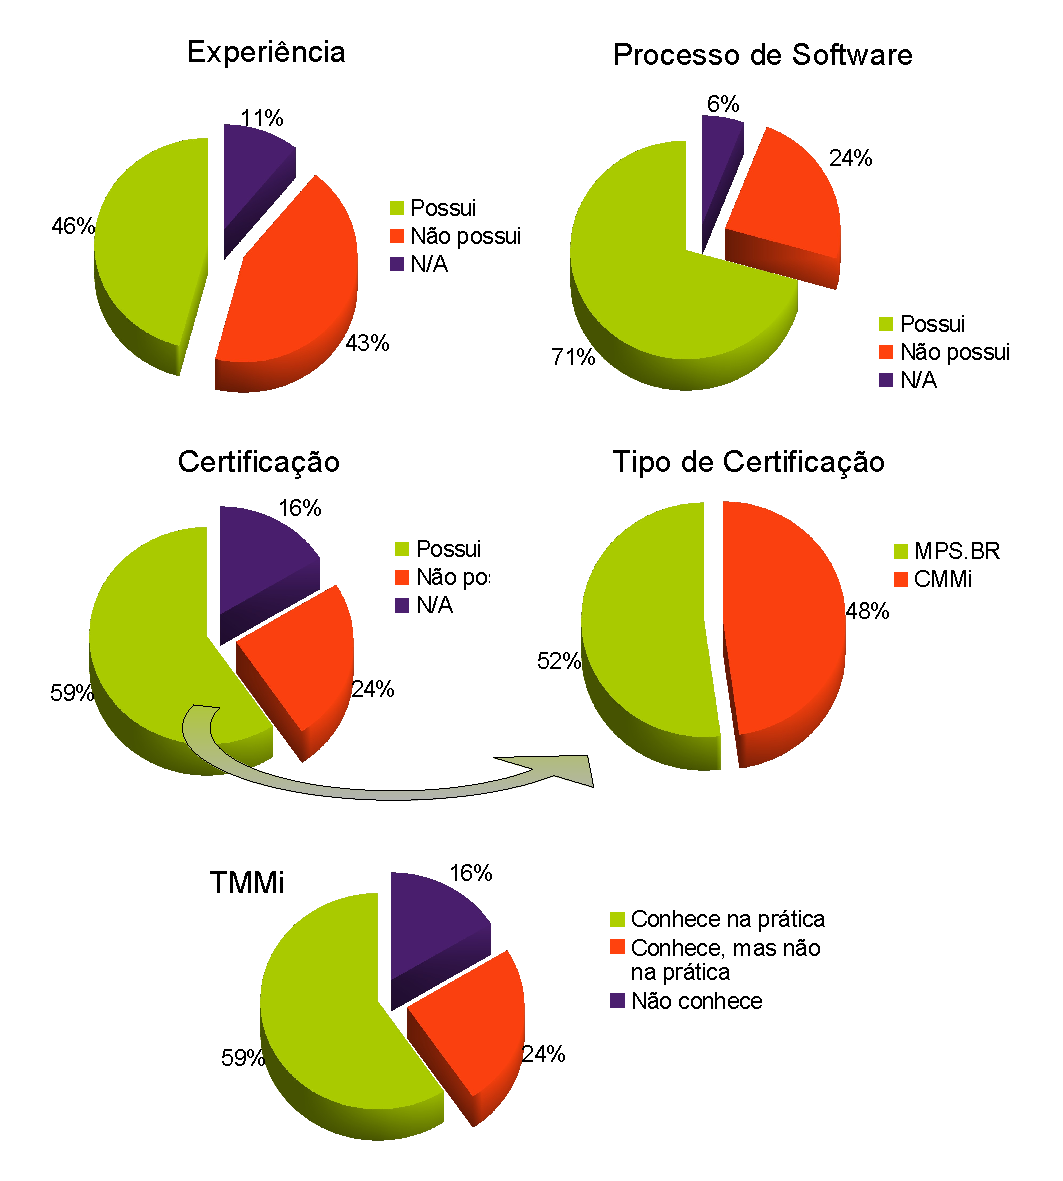
\includegraphics[width=.9\textwidth]{figures/chartsProfiles.pdf}
  \caption{Perfis obtidos na amostra \label{fig:chartsProfiles}}
\end{figure}


Lorem ipsum dolor sit amet, consectetur adipiscing elit. Sed consequat risus a enim iaculis et posuere metus adipiscing. Aliquam risus erat, elementum ut placerat vel, posuere vitae augue. Proin ac mattis ligula. Sed metus lectus, venenatis ac porta tristique, placerat non quam. Sed sit amet sem eu massa euismod condimentum. Praesent eget nulla id ligula luctus ultricies sit amet eu massa. Curabitur bibendum purus non ante tempus gravida eleifend urna aliquet. Fusce dolor nisl, ullamcorper nec dignissim id, ultrices id lectus. Proin auctor eros vel nunc lobortis ut pretium lectus tempus. Vestibulum lacinia gravida eros, quis tempus odio dapibus eu. Cras lobortis odio augue, eu molestie massa. Proin ac leo leo, ac lobortis est. Maecenas et aliquet sapien. Proin tempus viverra dui id lobortis.

Praesent neque erat, malesuada quis consequat quis, dapibus et sem. Curabitur est risus, fermentum eu consequat nec, sagittis vel ante. Phasellus odio lectus, tempus vitae pulvinar a, placerat et nisi. Maecenas ac lacus justo. Nunc accumsan iaculis quam, non sollicitudin dui volutpat sed. Donec suscipit adipiscing ultricies. Curabitur ac sapien ut mi facilisis porta. Pellentesque mattis orci et lorem mattis tincidunt. Aenean urna orci, porta id vestibulum at, fringilla id risus. Ut a mauris purus, at aliquet nibh. Sed ullamcorper ornare tellus non condimentum. Fusce elit mauris, laoreet nec hendrerit ut, varius ac turpis. Phasellus ut purus nisl. Nam volutpat sapien ac quam egestas lobortis.

Fusce non mauris ante. Integer vitae urna justo, quis faucibus libero. In commodo velit vitae nibh eleifend tristique tincidunt turpis auctor. Quisque nec porttitor mauris. Ut pharetra erat eu magna iaculis interdum. Vivamus tristique egestas ipsum vel placerat. Proin vulputate tempor nulla, venenatis vehicula lectus volutpat in. Maecenas nec risus nunc, sit amet sagittis lorem. Nunc pharetra viverra dolor et rutrum. Nulla facilisi. In sodales mollis nibh sit amet ultrices. Fusce eget fermentum orci. Nulla in sem sed massa mollis lobortis in eu massa. Donec ut aliquam velit. Maecenas imperdiet, eros et suscipit ornare, lorem justo consectetur libero, et bibendum nibh elit vitae turpis. Class aptent taciti sociosqu ad litora torquent per conubia nostra, per inceptos himenaeos. Nam aliquam convallis nulla, at hendrerit nibh condimentum a. Nullam euismod sagittis ligula, quis feugiat tellus dignissim quis.

\subsection{Subse��o de exemplo}

Lorem ipsum dolor sit amet, consectetur adipiscing elit. Cras at dui ligula. Vivamus eget est nulla. Suspendisse ligula elit, tempor ut facilisis vitae, mattis vitae ligula. Curabitur facilisis tempor nunc, eu vehicula neque tristique non. Aenean pellentesque odio non leo semper fringilla. Morbi semper, libero eu scelerisque egestas, tortor leo adipiscing lectus, quis molestie odio odio eu augue. Etiam mattis mi eu odio pellentesque imperdiet. Integer ac blandit elit. Maecenas elementum nunc id enim pellentesque consectetur. Phasellus porttitor iaculis enim sed consequat. Mauris scelerisque lacus nec nibh tempor in mattis urna tempus. Integer condimentum hendrerit ante nec commodo. Mauris suscipit, arcu et faucibus pretium, purus velit egestas purus, nec venenatis elit mauris nec ligula. Praesent lectus risus, consequat sit amet rutrum et, cursus in tellus.

\subsubsection{Subsubse��o de exemplo}

Lorem ipsum dolor sit amet, consectetur adipiscing elit. Cras at dui ligula. Vivamus eget est nulla. Suspendisse ligula elit, tempor ut facilisis vitae, mattis vitae ligula. Curabitur facilisis tempor nunc, eu vehicula neque tristique non. Aenean pellentesque odio non leo semper fringilla. Morbi semper, libero eu scelerisque egestas, tortor leo adipiscing lectus, quis molestie odio odio eu augue. Etiam mattis mi eu odio pellentesque imperdiet. Integer ac blandit elit. Maecenas elementum nunc id enim pellentesque consectetur. Phasellus porttitor iaculis enim sed consequat. Mauris scelerisque lacus nec nibh tempor in mattis urna tempus. Integer condimentum hendrerit ante nec commodo. Mauris suscipit, arcu et faucibus pretium, purus velit egestas purus, nec venenatis elit mauris nec ligula. Praesent lectus risus, consequat sit amet rutrum et, cursus in tellus.

\section{Outra se��o}

Lorem ipsum dolor sit amet, consectetur adipiscing elit. Proin euismod risus sed velit congue vitae posuere risus condimentum. Aliquam interdum condimentum risus, vel aliquet nibh pretium at. Integer egestas, dolor eget ultrices gravida, turpis nunc suscipit erat, ut aliquam velit nisl in turpis. Nam vel sodales justo. Nulla auctor, quam sed porta hendrerit, mi tortor rutrum ipsum, sed ullamcorper nisl erat nec ipsum. Class aptent taciti sociosqu ad litora torquent per conubia nostra, per inceptos himenaeos. Etiam eget arcu id nisi auctor iaculis. Curabitur dignissim porta lacus. Curabitur bibendum aliquet diam vel tempor. Maecenas vulputate aliquet purus eget interdum. Etiam pretium tortor in mi interdum volutpat.

Aenean at convallis lectus. Nulla adipiscing massa eget diam consequat a consequat nisi pharetra. Suspendisse potenti. Sed at tellus metus, at tempor turpis. Curabitur vitae ligula libero, et aliquet diam. Proin bibendum hendrerit interdum. Curabitur luctus, augue sit amet pharetra consectetur, erat tellus sagittis ligula, eget rhoncus neque diam mattis urna. Donec consequat pretium euismod. Nam pellentesque facilisis quam et scelerisque. Aenean eu lacus ac sem vehicula laoreet a quis erat.

Nulla facilisi. Sed a tortor eros, et viverra felis. Duis molestie elit in arcu condimentum quis blandit justo fermentum. Integer rhoncus accumsan hendrerit.

\chapter{Introdu��o}

Este cap�tulo introduz o contexto e a motiva��o que levaram � elabora��o de uma proposta ...

Teste de Acr�nimo (TdA)\acronym{TdA}{Teste de Acr�nimo}

\section{Contexto e Motiva��o}

Exemplos de cita��o:

\begin{itemize}
  \item Normal: \cite{Rodrigues2010}
  \item Autores fora dos par�nteses: \citeonline{Rodrigues2010}
\end{itemize}






\chapter{Outro Cap�tulo}


Este cap�tulo...



\section{Exemplo de Se��o}

Exemplo de figura: Na Figura~\ref{fig:chartsProfiles} ilustra-se ...


\begin{figure}[!ht]
%\begin{figure}[t]
  \centering
  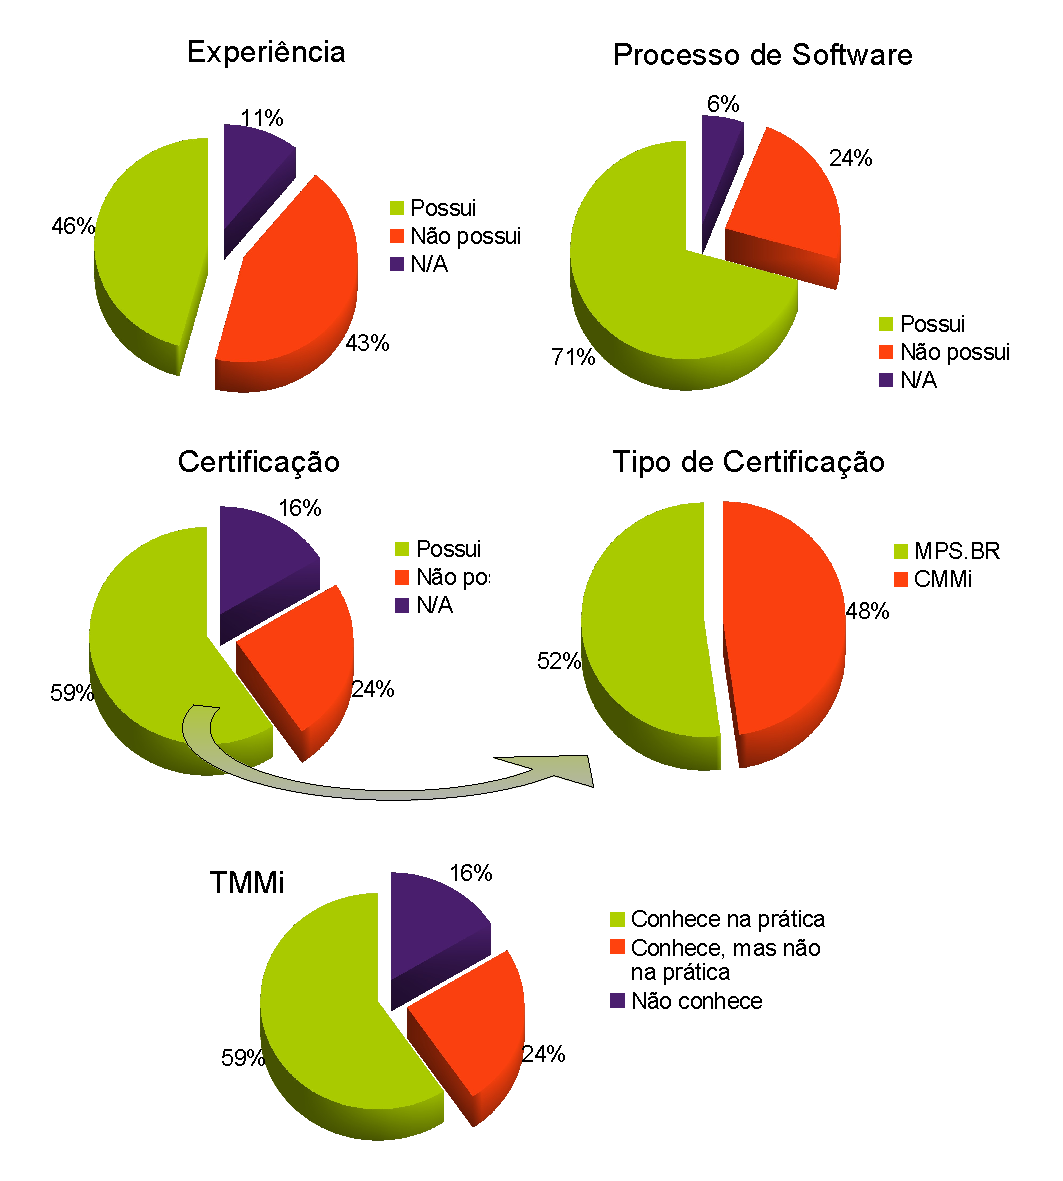
\includegraphics[width=.9\textwidth]{figures/chartsProfiles.pdf}
  \caption{Perfis obtidos na amostra \label{fig:chartsProfiles}}
\end{figure}


Lorem ipsum dolor sit amet, consectetur adipiscing elit. Sed consequat risus a enim iaculis et posuere metus adipiscing. Aliquam risus erat, elementum ut placerat vel, posuere vitae augue. Proin ac mattis ligula. Sed metus lectus, venenatis ac porta tristique, placerat non quam. Sed sit amet sem eu massa euismod condimentum. Praesent eget nulla id ligula luctus ultricies sit amet eu massa. Curabitur bibendum purus non ante tempus gravida eleifend urna aliquet. Fusce dolor nisl, ullamcorper nec dignissim id, ultrices id lectus. Proin auctor eros vel nunc lobortis ut pretium lectus tempus. Vestibulum lacinia gravida eros, quis tempus odio dapibus eu. Cras lobortis odio augue, eu molestie massa. Proin ac leo leo, ac lobortis est. Maecenas et aliquet sapien. Proin tempus viverra dui id lobortis.

Praesent neque erat, malesuada quis consequat quis, dapibus et sem. Curabitur est risus, fermentum eu consequat nec, sagittis vel ante. Phasellus odio lectus, tempus vitae pulvinar a, placerat et nisi. Maecenas ac lacus justo. Nunc accumsan iaculis quam, non sollicitudin dui volutpat sed. Donec suscipit adipiscing ultricies. Curabitur ac sapien ut mi facilisis porta. Pellentesque mattis orci et lorem mattis tincidunt. Aenean urna orci, porta id vestibulum at, fringilla id risus. Ut a mauris purus, at aliquet nibh. Sed ullamcorper ornare tellus non condimentum. Fusce elit mauris, laoreet nec hendrerit ut, varius ac turpis. Phasellus ut purus nisl. Nam volutpat sapien ac quam egestas lobortis.

Fusce non mauris ante. Integer vitae urna justo, quis faucibus libero. In commodo velit vitae nibh eleifend tristique tincidunt turpis auctor. Quisque nec porttitor mauris. Ut pharetra erat eu magna iaculis interdum. Vivamus tristique egestas ipsum vel placerat. Proin vulputate tempor nulla, venenatis vehicula lectus volutpat in. Maecenas nec risus nunc, sit amet sagittis lorem. Nunc pharetra viverra dolor et rutrum. Nulla facilisi. In sodales mollis nibh sit amet ultrices. Fusce eget fermentum orci. Nulla in sem sed massa mollis lobortis in eu massa. Donec ut aliquam velit. Maecenas imperdiet, eros et suscipit ornare, lorem justo consectetur libero, et bibendum nibh elit vitae turpis. Class aptent taciti sociosqu ad litora torquent per conubia nostra, per inceptos himenaeos. Nam aliquam convallis nulla, at hendrerit nibh condimentum a. Nullam euismod sagittis ligula, quis feugiat tellus dignissim quis.

\subsection{Subse��o de exemplo}

Lorem ipsum dolor sit amet, consectetur adipiscing elit. Cras at dui ligula. Vivamus eget est nulla. Suspendisse ligula elit, tempor ut facilisis vitae, mattis vitae ligula. Curabitur facilisis tempor nunc, eu vehicula neque tristique non. Aenean pellentesque odio non leo semper fringilla. Morbi semper, libero eu scelerisque egestas, tortor leo adipiscing lectus, quis molestie odio odio eu augue. Etiam mattis mi eu odio pellentesque imperdiet. Integer ac blandit elit. Maecenas elementum nunc id enim pellentesque consectetur. Phasellus porttitor iaculis enim sed consequat. Mauris scelerisque lacus nec nibh tempor in mattis urna tempus. Integer condimentum hendrerit ante nec commodo. Mauris suscipit, arcu et faucibus pretium, purus velit egestas purus, nec venenatis elit mauris nec ligula. Praesent lectus risus, consequat sit amet rutrum et, cursus in tellus.

\subsubsection{Subsubse��o de exemplo}

Lorem ipsum dolor sit amet, consectetur adipiscing elit. Cras at dui ligula. Vivamus eget est nulla. Suspendisse ligula elit, tempor ut facilisis vitae, mattis vitae ligula. Curabitur facilisis tempor nunc, eu vehicula neque tristique non. Aenean pellentesque odio non leo semper fringilla. Morbi semper, libero eu scelerisque egestas, tortor leo adipiscing lectus, quis molestie odio odio eu augue. Etiam mattis mi eu odio pellentesque imperdiet. Integer ac blandit elit. Maecenas elementum nunc id enim pellentesque consectetur. Phasellus porttitor iaculis enim sed consequat. Mauris scelerisque lacus nec nibh tempor in mattis urna tempus. Integer condimentum hendrerit ante nec commodo. Mauris suscipit, arcu et faucibus pretium, purus velit egestas purus, nec venenatis elit mauris nec ligula. Praesent lectus risus, consequat sit amet rutrum et, cursus in tellus.

\section{Outra se��o}

Lorem ipsum dolor sit amet, consectetur adipiscing elit. Proin euismod risus sed velit congue vitae posuere risus condimentum. Aliquam interdum condimentum risus, vel aliquet nibh pretium at. Integer egestas, dolor eget ultrices gravida, turpis nunc suscipit erat, ut aliquam velit nisl in turpis. Nam vel sodales justo. Nulla auctor, quam sed porta hendrerit, mi tortor rutrum ipsum, sed ullamcorper nisl erat nec ipsum. Class aptent taciti sociosqu ad litora torquent per conubia nostra, per inceptos himenaeos. Etiam eget arcu id nisi auctor iaculis. Curabitur dignissim porta lacus. Curabitur bibendum aliquet diam vel tempor. Maecenas vulputate aliquet purus eget interdum. Etiam pretium tortor in mi interdum volutpat.

Aenean at convallis lectus. Nulla adipiscing massa eget diam consequat a consequat nisi pharetra. Suspendisse potenti. Sed at tellus metus, at tempor turpis. Curabitur vitae ligula libero, et aliquet diam. Proin bibendum hendrerit interdum. Curabitur luctus, augue sit amet pharetra consectetur, erat tellus sagittis ligula, eget rhoncus neque diam mattis urna. Donec consequat pretium euismod. Nam pellentesque facilisis quam et scelerisque. Aenean eu lacus ac sem vehicula laoreet a quis erat.

Nulla facilisi. Sed a tortor eros, et viverra felis. Duis molestie elit in arcu condimentum quis blandit justo fermentum. Integer rhoncus accumsan hendrerit.



%% coloque aqui o seu arquivo .bib
%% IMPORTANTE: nao use bibliographystyle!
%% o estilo ja vem definido.
\bibliography{references}

%% de acordo com o template, o glossario vem
%% depois das referencias e deve estar em ordem
%% alfabetica.
%% depois de muito esforco consegui fazer com que
%% o glossario ficasse em ordem alfabetica automaticamente.
%% ainda nao sei a escalabilidade do algoritmo :(

%% DICA: voce pode ir definindo os acronimos ao longo do texto.
%% Por exemplo, no capitulo 1, vc ta escrevendo:
%% Segundo Fulano, Model-Driven Development (MDD)\acronym{MDD}{Model-Driven Development} � uma t�cnica bla bla bla...


\acronym{PISO}{Polo das Ind�strias de Software}
\acronym{MPT.Br}{Melhoria do Processo de Teste de Software Brasileiro}
\acronym{MPS.Br}{Melhoria do Processo de Software Brasileiro}
\acronym{TMMi}{Test Maturity Model integration}
\acronym{CMMI}{Capability Maturity Model Integration}
\acronym{KITMap}{Knowledge and Improvement Map}
\acronym{KITTool}{Knowledge and Improvement on Test Tool}
\acronym{PA}{Process Area}
\acronym{SG}{Specific Goal}
\acronym{SP}{Specific Pratic}

\listofacronyms

% \apendice

% \chapter{Explica��o do que � ap�ndice}
% 
% \begin{resumocap}
% D� pra usar o resuminho aqui tamb�m.
% \end{resumocap}
% 
% Segundo a norma, ap�ndice � um documento elaborado pelo autor a fim de complementar sua argumenta��o sem afetar a unidade nuclear do trabalho.
% 
% \chapter{Outro ap�ndice}
% 
% S� pra ilustrar mais de um ap�ndice.

% \anexo
%\chapter{Tabela de Depend�ncias}
\label{chap:anexoA}


Este anexo apresenta uma tabela de depend�ncias... 



\begin{table}[htp]
 
\fontencoding{T1}
\fontfamily{\sfdefault}
\fontseries{m}
\fontshape{n}
\fontsize{8}{14}
\selectfont

\begin{tabular}{|p{7.2cm}|c|p{7.0cm}|}

  
  %\multicolumn{3}{c}{Pr�tica \hfill Depend�ncia \hfill Pr�tica}\\ \hline

  \hline

  \multicolumn{1}{|c}{\textbf{Pr�tica}} & \multicolumn{1}{|c}{\textbf{Dep}} & \multicolumn{1}{|c|}{\textbf{Pr�tica}} \\ \hline\hline




\multirow{4}{*}{Analisar riscos do produto}	&	N	&	Definir a abordagem de teste	\\ 

	&	N	&	Identificar e priorizar casos de teste	\\

	&	N	&	Identificar e priorizar condicoes de teste	\\ 

	&	N	&	Identificar elementos e caracteristicas a serem testados	\\ \hline




\end{tabular} 

%\end{footnotesize}

\caption{Depend�ncias entre pr�ticas do TMMi identificadas por \citeonline{Hohn}, sendo que N representa depend�ncia \emph{necess�ria} e A representa depend�ncia de \emph{alinhamento}. \label{tab:dependencias}}


\end{table}







\end{document}